%-------------------------------------------------------------------------------

% This file is part of code_saturne, a general-purpose CFD tool.
%
% Copyright (C) 1998-2024 EDF S.A.
%
% This program is free software; you can redistribute it and/or modify it under
% the terms of the GNU General Public License as published by the Free Software
% Foundation; either version 2 of the License, or (at your option) any later
% version.
%
% This program is distributed in the hope that it will be useful, but WITHOUT
% ANY WARRANTY; without even the implied warranty of MERCHANTABILITY or FITNESS
% FOR A PARTICULAR PURPOSE.  See the GNU General Public License for more
% details.
%
% You should have received a copy of the GNU General Public License along with
% this program; if not, write to the Free Software Foundation, Inc., 51 Franklin
% Street, Fifth Floor, Boston, MA 02110-1301, USA.

%-------------------------------------------------------------------------------

\nopagebreak

\section{Extended cell neighbourhood}

The neighbourhood is defined as the collection of cells $J_i$ around the
cell $I$ under consideration for various algorithms.

We consider:

\begin{itemize}
  \item the \emph{standard} neighborhhod, containing all cells sharing
        a face with $I$.
  \item the \emph{extended} neighborhhod, containing a subset of cells sharing
        a vertex with $I$, and excluding the standard neighborhood.
\end{itemize}

The standard neighbourhood is used in most finite volume operators, whether
computing fluxes and balances, or in gradient reconstruction.

The extended neighborhood may be used to supplement the base neighborhood
when using least-squares gradient reconstruction, so as to obtain a smoother
and more stable result in the case of significant face non-orthogonality
of offset (which is always the case with tetrahedral meshes, and may be the
case with strongly distorted hexahedra).

It may also be used for some other smoothing operations, such as LES filters
or other smoothing operators (though it is recommended to use another approach
for operators not akin to gradients, so that tuning for gradients does not
interfere with those operators).

\subsection{Reduced extended neighborhood}

Whereas the standard neighborhood usually 6 cells for hexahedra and
4 for tetrahedra, the matching extended neighborhood contains 20 cells
(26 - 6) for hexahedra, and often more than 60 cells on average for tetrahedra
(some tetrahedra may even have more than 150 neighbors).
So accessing and computing values based on this neighborhood can be quite
expensive.

So when possible, we will use a reduced (more precisely, restricted) extended
neighborhood, including only a subset of a cell's vertex-adjacent neighbors,
so as to improve performance.

Several algorithms for such reduction are possible (see the user guide).

The simplest one selects cells with centers best aligned opposite to face-adjacent
cell centers, and discards others, leading to a number of additional cells in
the extended neighbourhood at most equal to the number of cell faces. Using this
restriction significantly improves stability with tetradral meshes compared with
using only the standard neighborhood, with little additional cost, but does
not provide the same robustness as using the full neighbourhood.

Another optimized neighbourhood reduction (restriction) algorithm based on
heuristics provides better robustness, at a reasonable additional cost
(much faster than using the complete extended neighborhood) is described
in the next section.

\section{Optimized (heuristics) neighbourhood}

\subsection{Principle}

This optimized neighbourhood is designed to:
\begin{itemize}
  \item have a calculation cost
    reduced compared to full neighbourhood (all the cells sharing at least
    one vertex with the cell $I$ under consideration) by selecting only
    some cells in the full neighbourhood and
  \item minimise both the offset of the neighbourhood
    $|| \underline{IC} ||$ and the average distance of the neighbours.
\end{itemize}

The optimized neighbourhood is also designed to improve a weakness
of the full neighbourhood: a tendency to produce more prominent
spurious modes (repeated non physical jumps of a given quantity passing
from one cell to another) than the restricted neighbourhood (all the cells
sharing at least one face with the cell $I$ under consideration).
The spurious modes appear in regular hexahedral or prismatic portions
of the mesh where the restricted neighbourhood is stable enough. The
optimized neighbourhood has a criterion to detect these zones
and if the criterion is met it switches to a restricted neighbourhood.

Moreover, the optimized neighbourhood will keep all the cells in the full
neighbourhood if the cell $I$ has a very large aspect ratio.

Finally, at the boundary, the default behaviour is also to keep the restricted
neighbourhood, only the cells with more than one boundary face will use more
neighbours. These choices come from numerical experiments.

\subsection{Implementation}

First, the cell type is deduced from the number of triangles and quadrangles
of the cell $I$. For example, a cell with 6 quadrangles only is assumed to be
a hexahedra, while a cell with 2 triangles and 3 quadrangles is assumed to be
a prism, and one with 4 triangles a tetrahedra.

\begin{remark}
In rare cases, a cell with 2 triangles and 3 quadrangles might be a tetrahedron
with a split face, as cells in figure \ref{fig:false_prism}), but this is rare
(expected to occur only when an initial face is subdivided through a mesh joining
operation), so we prefer to keep tests simple, for better performance.

\begin{figure}[h]
  \centering
  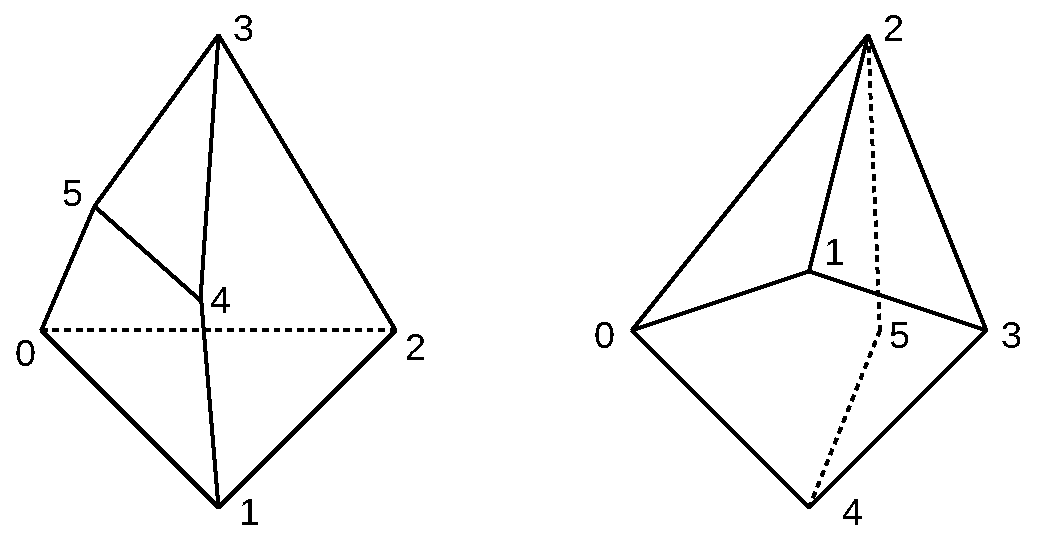
\includegraphics[width=0.3\linewidth]{cell_type_2_t_3_q.pdf}
  \caption{Tetrahedra with split face: degenerate and false prism}
  \label{fig:false_prism}
\end{figure}
\end{remark}

Second, the center of gravity of the restricted neighbourhood $C$ is calculated
together with the average distance of the cells in the restricted neighbourhood.
Also, if the cell is identified as an hexahedra or a prism,
the following regularity criterion is calculated for each face\footnote{only
triangles face in case of a prism since a prismatic mesh is assumed to possibly
be regular only in the direction normal to the triangle faces}:

\begin{equation}
  r_{crit} = \underline{IF}.\underline{FJ}
  - 0.9 \, ||\underline{IF}|| \, ||\underline{FJ}||
  \label{eqn:reg_crit}
\end{equation}

If for all faces the criterion is $>0$ then the mesh is considered to be locally regular
and only the restricted neighbourhood will be retained.

Another geometric criterion has an impact on the retained neighbourhood, the
aspect ratio defined as follow:

\begin{equation}
  ar = \frac{6\,\Omega^{2/3}}{\sum_{n_F} S}
  \label{eqn:aspect_r}
\end{equation}

Obviously for a cube, $ar = 1$. For a rectangular solid with an height a hundred
times smaller than the base, $ar = 0.1365$. Any cell with $ar < 0.1365$ will have
the full neighbourhood activated.

The last part of the code is the definition of the optimized neighbourhood for
cells that are not ``regular'' nor ``too flat''.

Inside a loop on the cells in the extended neighbourhood only,
the cell $J_i$ which minimises the sum of the updated offset $\underline{IC}$
and its distance to the cell $I$ is selected. With $n$ the number
of cells already in the neighbourhood (restricted included) it writes

\begin{equation}
  \mbox{argmin} \left(\left||n\underline{IC_{}}+(n+2)\underline{IJ_i}\right||\right)
  \label{eqn:loc_crit}
\end{equation}

After that, both the offset $\underline{IC}$ and the average length of the
selected cells $\overline{||\underline{IJ_i}||}$
are updated. Then, if the total number of cells retained inside the
extended neighbourhood reaches a min value fixed at 10 in the code and if
the new selected cell $J_i$ improves the neighbourhood, the whole set of
cells already selected is retained.

The improvement of the neighbourhood is written as:

\begin{equation}
  \left( ||\underline{IC_{}}|| + 0.1\,\Omega^{1/3} \right) \, \overline{||\underline{IJ_i}||}
  \label{eqn:crit}
\end{equation}

Also, as soon as the offset $||\underline{IC}||$ is small enough ($ < 0.01\, \Omega^{1/3}$)
the search for new ``optimal'' neighbours is stopped.

\subsection{Suggested improvements}

\begin{itemize}

\item There is a possibility that the degenerated or false prism on figure
\label{fig:false_prism} appears as a regular prism. This would be unfortunate
because such a cell would be of very poor quality and would need more than the
restricted neighbourhood. Further geometric tests could detect this.

\item Selecting $n_s$ cells among the $n_e$ ones in the full neighbourhood that
collectively minimise the average distance and the neighbourhood offset is
probably $NP$ hard (it looks similar to the Travelling Salesman Problem - TSP).
\textit{A priori} we are only able to solve it with an heuristic. The
approach used here is the most simple one, more clever algorithms are
possible and could be studied. A first step could be for the cells $I$
where the neighbourhood offset stays high to switch from
finding the one cell $J$ that minimises (\ref{eqn:loc_crit}) to
finding the pair of cells $J$ that minimises (\ref{eqn:loc_crit}). This might
be reminiscent of the $k-opt$ algorithms in the TSP.

\item Globally many aspects of this code are ``heuristic'' perhaps more
formal/satisfactory definitions would be possible.

\end{itemize}
